\documentclass[11pt,a4paper]{article}
\usepackage[french]{babel}
\usepackage[utf8]{inputenc}
\usepackage[T1]{fontenc}
\usepackage{graphicx}
\usepackage{amsmath, amssymb}
\usepackage{hyperref}
\usepackage{geometry}
\usepackage{float}
\usepackage{tikz}
\usepackage{setspace}
\usepackage{titlesec}
\usepackage{enumitem}
\usepackage{amsthm}

\usetikzlibrary{positioning,shapes,arrows}

% 设置页边距
\geometry{margin=2cm}

% 设置段落间距和缩进
\setlength{\parskip}{0.5em}
\setlength{\parindent}{0em}

% 设置行距
\onehalfspacing

% 设置标题间距
\titlespacing*{\section}{0pt}{0.5em}{0.3em}
\titlespacing*{\subsection}{0pt}{0.3em}{0.2em}

% 设置列表间距
\setlist[itemize]{noitemsep, topsep=0pt, parsep=0pt, partopsep=0pt}
\setlist[enumerate]{noitemsep, topsep=0pt, parsep=0pt, partopsep=0pt}

\title{Projet : Couverture de graphe (Vertex Cover)\\
UE Complexité -- M1 Informatique, Sorbonne Université}
\author{Yuxiang ZHANG \\ Kenan ALSAFAD}
\date{Année universitaire 2025-2026}

\begin{document}
\maketitle

\section{Introduction}

Le problème de \textit{couverture de graphe} (\textit{Vertex Cover}) est un problème fondamental en théorie des graphes et en optimisation combinatoire.  
Étant donné un graphe non orienté $G = (V, E)$, une \textbf{couverture de sommets} est un sous-ensemble $V' \subseteq V$ tel que chaque arête $e \in E$ ait au moins une extrémité dans $V'$.  
L'objectif est de trouver une couverture de taille minimale.

Ce problème est \textbf{NP-difficile}. Sa version décisionnelle, consistant à déterminer s'il existe une couverture de taille au plus $k$, est \textbf{NP-complète}.  
Le but de ce projet est d'implémenter plusieurs approches — exactes et approchées — permettant de résoudre ce problème, et d'en analyser les performances empiriques.

\section{Représentation du graphe}

\subsection{Structure de données}
Le graphe est représenté par une \textbf{liste d’adjacence} sous forme de dictionnaire Python :
\[
\text{adj} = \{\,v : [\,\text{voisins de } v\,]\,\},
\]
offrant un bon compromis entre accès rapide et mémoire, particulièrement pour des graphes clairsemés.  
Cette structure est encapsulée dans la classe \texttt{Graph}, qui fournit toutes les opérations nécessaires.

\subsection{Lecture et génération de graphes}
\begin{itemize}
    \item \texttt{read\_graph(filename)} : lit un fichier texte et construit la liste d’adjacence pour un graphe non orienté.
    \item \texttt{generate\_random\_graph(n, p)} : génère un graphe aléatoire selon le modèle Gilbert–Erdős–Rényi $G(n,p)$, utile pour les tests expérimentaux.
\end{itemize}

\subsection{Opérations de base}
La classe \texttt{Graph} implémente :
\begin{itemize}
    \item Suppression d’un ou plusieurs sommets (\texttt{remove\_vertex}, \texttt{remove\_vertices}, \texttt{remove\_vertices\_inplace}) ;
    \item Calcul des degrés (\texttt{degree}, \texttt{degrees\_dict}, \texttt{degrees\_list}) et sommet(s) de degré maximal (\texttt{max\_degree\_vertex}) ;
    \item Copie indépendante du graphe (\texttt{copy}) pour certaines heuristiques.
\end{itemize}

Ces opérations constituent la base pour l’implémentation des heuristiques de couverture présentées dans la section suivante.


\section{Méthodes approchées}

\subsection{Algorithme glouton}

L'algorithme glouton sélectionne itérativement les sommets de degré maximal :

\begin{enumerate}
    \item Tant qu'il reste des arêtes non couvertes :
    \begin{enumerate}
        \item Identifier le sommet de degré maximal
        \item Ajouter ce sommet à la couverture $C$
        \item Supprimer ce sommet du graphe
    \end{enumerate}
\end{enumerate}

\subsubsection{Non-optimalité du glouton}

\paragraph{Contre-exemple:}

Considérons 5 sommets notés \(a,b,c,d,e\), les arêtes sont \((a,b),(b,c),(c,d),(d,e)\) :
\begin{figure}[H]
    \centering
    \begin{tikzpicture}[scale=1, every node/.style={circle, draw, fill=white, inner sep=1.5pt, minimum size=7mm}]
        % Positions des sommets (ligne)
        \node (a) at (-2,0) {a};
        \node (b) at (-1,0) {b};
        \node (c) at (0,0)  {c};
        \node (d) at (1,0)  {d};
        \node (e) at (2,0)  {e};

        % Arêtes (chemin)
        \draw (a) -- (b);
        \draw (b) -- (c);
        \draw (c) -- (d);
        \draw (d) -- (e);
    \end{tikzpicture}
\end{figure}

\textbf{Exécution de l'algorithme glouton (stratégie : sommet de degré maximal).}  
Les degrés sont : $\deg(a)=1,\ \deg(b)=2,\ \deg(c)=2,\ \deg(d)=2,\ \deg(e)=1$.  
Supposons que le critère de bris d'égalité amène l'algorithme à choisir le sommet central \(c\) (un sommet de degré maximal). Alors :
\begin{enumerate}
  \item On ajoute \(c\) à la couverture : $C=\{c\}$.
  \item On supprime \(c\) et toutes ses arêtes incidentes : les arêtes $(b,c)$ et $(c,d)$ disparaissent.
  \item Il reste les arêtes $(a,b)$ et $(d,e)$. Pour couvrir ces arêtes il faut au moins deux sommets supplémentaires (par exemple \(a\) et \(e\)).
\end{enumerate}
L'algorithme glouton retourne donc une couverture de taille $|C_{\text{glouton}}|=3$ (par exemple $\{c,a,e\}$).

\medskip

\textbf{Couverture optimale.}  
On vérifie que la paire $C^{*}=\{b,d\}$ couvre toutes les arêtes sont toutes couvertes par au moins un sommet dans $\{b,d\}$. Ainsi $|C^{*}|=2$.

Par conséquent, cet exemple montre concrètement que l'algorithme glouton « choisir le sommet de degré maximal » n'est pas optimal en général : il peut retourner une couverture strictement plus grosse que l'optimum.

\subsubsection{Non-r-approximation}

On construit un graphe arborescent $k$-aire sur $L$ niveaux pour montrer que l'algorithme glouton n'est pas $r$-approché pour aucune constante bornée $r$ :

\begin{itemize}
    \item Racine $v_0$ au niveau 0, connectée à $k$ sommets au niveau 1, chaque niveau suivant répète ce schéma jusqu’aux feuilles (niveau $L$).
    \item \textbf{Glouton} : couvre d’abord $v_0$, puis tous les sommets de niveau 1, et ainsi de suite jusqu’à ce que toutes les arêtes soient couvertes.
    \item \textbf{Optimal} : stratégie \emph{bottom-up}, en choisissant les parents des feuilles puis en remontant, minimisant ainsi le nombre de sommets.
\end{itemize}

Le nombre de sommets couvert par l’optimal croît beaucoup plus lentement que celui choisi par le glouton :
\[
|C_{\text{glouton}}| = 1 + k + k^2 + \dots + k^{L-1} = \frac{k^L - 1}{k-1},\quad
|C^*| = \sum_{i=0}^{\lfloor (L-1)/2 \rfloor} k^{L-1-2i}.
\]

Le ratio
\[
\frac{|C_{\text{glouton}}|}{|C^*|} = \frac{k^L - 1}{(k-1)\sum_{i=0}^{\lfloor (L-1)/2 \rfloor} k^{L-1-2i}}
\]
peut devenir arbitrairement grand lorsque $L\to\infty$ ou $k$ augmente.

\paragraph{Conclusion} L’algorithme glouton n’est pas $r$-approché pour aucune constante $r$ bornée.


\subsection{Méthode du couplage maximal}

L'algorithme du couplage maximal sélectionne des arêtes indépendantes et ajoute leurs deux sommets à la couverture :

\begin{enumerate}
    \item Pour chaque arête $(u,v)$ non couverte :
    \begin{enumerate}
        \item Si $u$ et $v$ ne sont pas dans la couverture, les ajouter
    \end{enumerate}
\end{enumerate}

Cet algorithme garantit une \textbf{2-approximation} : $|C| \leq 2|C^*|$.

\subsection{Comparaison des méthodes approchées}

\paragraph{Protocole et résultats}
Une comparaison systématique entre les algorithmes glouton et de couplage a été réalisée sur des graphes aléatoires $G(n,0.3)$ pour $n$ variant de 55 à 547. Le protocole inclut la détermination de la taille maximale $N_{\max}=547$ permettant un temps d'exécution raisonnable ($\leq$3s), avec 10 instances par taille pour lisser les mesures.

\begin{figure}[H]
    \centering
    \begin{minipage}{0.49\textwidth}
        \centering
        \includegraphics[width=\textwidth]{courbes_temps.png}
        \caption{Temps d'exécution (échelle log-log)}
    \end{minipage}
    \hfill
    \begin{minipage}{0.49\textwidth}
        \centering
        \includegraphics[width=\textwidth]{comparaison_couvertures.png}
        \caption{Taille des couvertures}
    \end{minipage}
    \label{fig:exp_comparaison}
\end{figure}

\paragraph{Analyse des performances}
Les résultats expérimentaux confirment les complexités théoriques :
\begin{itemize}
    \item \textbf{Temps :} L'algorithme de couplage ($O(n+m)$) est significativement plus rapide que le glouton ($O(n^2)$), comme le montre la pente plus faible en échelle log-log
    \item \textbf{Qualité :} Les deux algorithmes produisent des solutions de taille comparable sur graphes aléatoires, bien que le couplage offre une garantie théorique de 2-approximation
    \item \textbf{Compromis :} Le couplage combine efficacité et garanties théoriques, tandis que le glouton, bien que légèrement plus lent, maintient une excellente qualité pratique
\end{itemize}

Cette analyse valide le choix de l'algorithme de couplage pour des applications nécessitant à la fois rapidité et garanties de performance.

\section{S\'eparation et \'evaluation}

\subsection{Branchement simple}

Le branchement consid\'er\'e est le suivant. \'Etant donn\'e un graphe $G$ et un ensemble
de sommets $C$ initialement vide, on choisit une ar\^ete $e=\{u,v\}$ et on d\'eveloppe deux
branches :
\begin{itemize}
  \item on suppose $u\in C$ et on r\'esout le probl\`eme sur $G\setminus\{u\}$ ;
  \item on suppose $v\in C$ et on r\'esout le probl\`eme sur $G\setminus\{v\}$.
\end{itemize}

Cette recherche exhaustrice produit un arbre de branchement explor\'e en profondeur.  
Dans notre code la m\'ethode correspondante s'appelle \texttt{branchement\_simple()} et utilise
une \textbf{pile} pour g\'erer les nœuds de l’arbre (structure LIFO) ; chaque \'etat sur la
pile est un couple \texttt{(remaining\_edges, current\_solution)}. Pour limiter la surcharge
m\'emoire nous ne stockons pas une copie compl\`ete du graphe \`a chaque nœud mais la liste
des ar\^etes restantes et l’ensemble partiel de sommets choisis. La m\'ethode renvoie la
meilleure couverture rencontr\'ee (\texttt{best\_C})
ainsi qu’un compteur du nombre de nœuds g\'en\'er\'es
(\texttt{nodes\_generated}).

\subsubsection{Vérification sur exemples simples}

Pour vérifier la validité de notre implémentation, nous avons comparé les résultats de l'algorithme de branchement avec ceux d'une recherche exhaustive par force brute. La fonction \texttt{bruteforce\_vertex\_cover(adj)} teste systématiquement tous les sous-ensembles de sommets par taille croissante, avec élagage précoce dès qu'une couverture optimale est trouvée.

\paragraph{Exemple 1 - Chemin à 5 sommets :}
\begin{verbatim}
Graphe : 0-1-2-3-4 (4 arêtes)
Force brute : {1, 3} (unique solution optimale, taille 2)
Branchement : {1, 3} (15 noeuds générés)
Validation : True
\end{verbatim}
\textbf{Analyse :} L'algorithme trouve l'unique couverture optimale, confirmant sa correction sur les graphes avec une seule solution optimale.

\paragraph{Exemple 2 - Graphe complet $K_4$ :}
\begin{verbatim}
Graphe : K4 (6 arêtes, 4 sommets)
Force brute : 4 solutions optimales de taille 3
  [{0,1,2}, {0,1,3}, {0,2,3}, {1,2,3}]
Branchement : {1, 2, 3} (15 noeuds générés)  
Validation : True
\end{verbatim}
\textbf{Analyse :} Le graphe complet $K_4$ admet plusieurs couvertures optimales. L'algorithme de branchement retourne l'une des solutions optimales, démontrant sa capacité à trouver des solutions valides même en présence de multiples optimums.

\subsubsection{Expérimentations et analyse de complexité}

\paragraph{Protocole expérimental}
Nous avons évalué les performances du branchement simple sur des graphes aléatoires $G(n,p)$ avec $n \in \{8,10,12,14,16\}$ et différentes densités ($p \in \{0.1,0.3,0.5,1/\sqrt{n}\}$). Pour chaque configuration, 3 instances ont été générées et nous avons mesuré le temps d'exécution, la taille des solutions et le nombre de nœuds générés.

\paragraph{Résultats et analyse}
Les résultats confirment la complexité exponentielle théorique $O(2^n)$ du branchement simple. L'analyse semi-log des temps d'exécution révèle une croissance linéaire, caractéristique des algorithmes exponentiels. La densité du graphe influence significativement les performances : les instances denses ($p=0.5$) montrent une complexité pratique plus élevée que les instances éparses ($p=0.1$).

\begin{figure}[H]
  \centering
  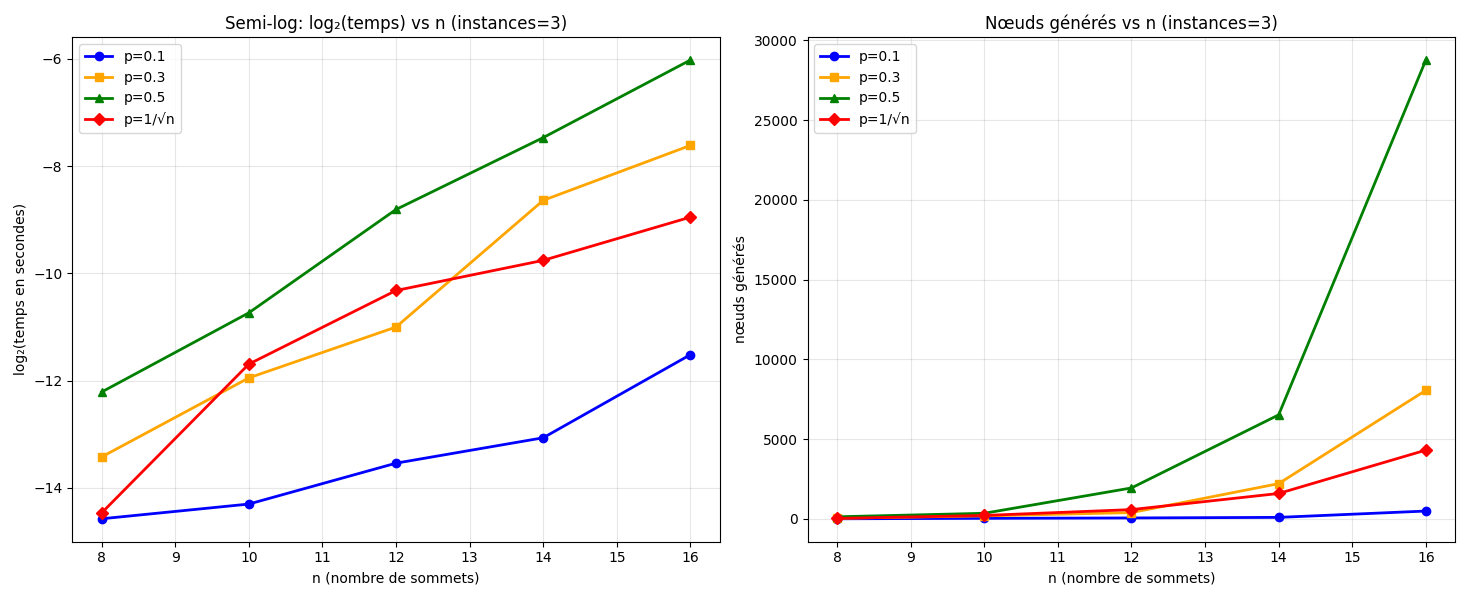
\includegraphics[width=0.8\linewidth]{Figure_1.png}
  \caption{Analyse de la complexité du branchement simple : croissance exponentielle du temps d'exécution et des nœuds généré}
  \label{fig:branchtime}
\end{figure}

\paragraph{Implications pratiques}
Bien que l'algorithme soit exact (100\% de solutions valides), sa complexité exponentielle limite son applicabilité à des instances de taille modérée ($n \leq 16$). L'extrapolation des tendances montre que pour $n=30$, le temps d'exécution dépasserait 8 minutes, justifiant le développement d'optimisations pour traiter des instances plus grandes.

\subsection{Ajout de bornes inférieures pour l'élagage}

Pour améliorer l'efficacité du branchement, on utilise des bornes inférieures permettant d'élaguer précocement les branches. Soit $G=(V,E)$ un graphe avec $|V|=n$, $|E|=m$, $\Delta$ le degré maximum, $M$ un couplage et $C$ une couverture de sommets. Alors :
\[
|C|\ge \max\{b_1,b_2,b_3\},\quad 
b_1=\Big\lceil\frac{m}{\Delta}\Big\rceil,\quad 
b_2=|M|,\quad 
b_3=\frac{2n-1-\sqrt{(2n-1)^2-8m}}{2}.
\]

\subsubsection{Démonstrations}

\paragraph{Borne $b_1=\lceil m/\Delta\rceil$}
Chaque sommet couvre au plus $\Delta$ arêtes, donc $\Delta|C|\ge m$, d'où $|C|\ge \lceil m/\Delta\rceil$.

\paragraph{Borne $b_2=|M|$}
Pour chaque arête $(u,v)\in M$, au moins un des sommets $u,v$ doit être dans $C$. Comme les arêtes de $M$ sont disjointes, il faut au moins $|M|$ sommets, donc $|C|\ge |M|$.

\paragraph{Borne $b_3=\frac{2n-1-\sqrt{(2n-1)^2-8m}}{2}$}
Si $|C|=k$, alors $V\setminus C$ est indépendant. Le graphe a au plus $k(n-k)$ arêtes entre les deux ensembles et $\binom{k}{2}$ à l’intérieur de $C$, donc :
\[
m\le k(n-k)+\frac{k(k-1)}{2}=kn-\frac{k^2+k}{2}.
\]
En multipliant par $2$ : $2m\le 2kn-k^2-k$, soit
\[
k^2-(2n-1)k+2m\le0.
\]
Le discriminant est $\Delta=(2n-1)^2-8m$. L’inégalité est vérifiée pour
\[
k\ge\frac{2n-1-\sqrt{(2n-1)^2-8m}}{2}=b_3.
\]
Ainsi, toute couverture vérifie $|C|\ge b_3$.

\subsubsection{Évaluation des stratégies d'optimisation}

\paragraph{Stratégies implémentées}
Conformément aux exigences du projet, nous avons évalué six stratégies combinant solutions réalisables (couplage et glouton) et bornes inférieures :
\begin{itemize}
  \item \textbf{Branchement Simple} : référence sans optimisation, servant de baseline avec complexité exponentielle
  \item \textbf{Branchement Couplage seul} : utilise uniquement la solution réalisable par couplage maximal
  \item \textbf{Branchement Bornes seules} : élagage exclusivement par les trois bornes inférieures
  \item \textbf{Branchement Couplage + bornes} : combinaison synergique recommandée
  \item \textbf{Branchement Glouton seul} : utilise la solution gloutonne comme réalisable initiale  
  \item \textbf{Branchement Glouton + bornes} : alternative combinant l'heuristique gloutonne avec l'élagage
\end{itemize}

\paragraph{Synthèse des performances}
L'évaluation comparative des six stratégies d'optimisation révèle des conclusions claires :

\begin{itemize}
  \item \textbf{Performance temporelle} : \textbf{Bornes seules} > \textbf{Couplage+bornes} > \textbf{Glouton+bornes} > \textbf{Couplage seul} > \textbf{Glouton seul} > \textbf{Branchement simple}
  
  \item \textbf{Réduction des nœuds} : Les stratégies avec bornes (\textbf{Couplage+bornes}, \textbf{Glouton+bornes}, \textbf{Bornes seules}) réduisent >85\% des nœuds explorés
\end{itemize}

\paragraph{Analyse conclusive}
\begin{itemize}
  \item Les \textbf{bornes inférieures} sont l'optimisation la plus efficace, réduisant drastiquement l'espace de recherche
  \item La combinaison avec des \textbf{solutions réalisables} améliore davantage l'élagage
  \item Le \textbf{couplage} est préférable au \textbf{glouton} pour sa complexité constante et sa qualité garantie
  \item Les stratégies sans bornes (\textbf{Couplage seul}, \textbf{Glouton seul}) offrent des gains limités
\end{itemize}

\begin{figure}[H]
  \centering
  \includegraphics[width=0.8\linewidth]{comparasion_tous.png}
  \caption{Comparaison des six stratégies de branchement : temps d'exécution et nœuds générés}
\end{figure}

\subsection{Amélioration du branchement (versions v1, v2, v3)}

\paragraph{Description des améliorations}
Nous avons développé trois versions améliorées du branchement, chacune introduisant des heuristiques spécifiques :

\begin{itemize}
  \item \textbf{Version 1 - Branchement asymétrique} : Évite la redondance en sélectionnant dans la seconde branche le sommet $v$ et tous les voisins de $u$, réduisant ainsi la symétrie dans l'arbre de recherche.
  
  \item \textbf{Version 2 - Sélection par degré maximal} : Améliore v1 en sélectionnant systématiquement l'arête contenant le sommet de degré maximal, maximisant la réduction du graphe à chaque étape.
  
  \item \textbf{Version 3 - Traitement optimal des sommets de degré 1} : Combine v2 avec un prétraitement agressif des sommets de degré 1, appliquant une règle d'optimalité locale avant le branchement principal.
\end{itemize}

Dans un graphe $G$, si un sommet $u$ est de degré 1, alors il existe toujours une couverture optimale qui ne contient pas $u$.

\paragraph{Preuve}
Soit $u$ un sommet de degré 1 et $v$ son unique voisin. Considérons deux cas :

\begin{enumerate}
    \item Si $v$ est dans la couverture optimale, alors l'arête $(u,v)$ est déjà couverte, donc $u$ n'est pas nécessaire.
    
    \item Si $v$ n'est pas dans la couverture optimale, alors pour couvrir l'arête $(u,v)$, nous devons inclure $u$.
\end{enumerate}

Cependant, si nous choisissons d'inclure $u$ dans la couverture, nous pouvons obtenir une couverture de même taille en remplaçant $u$ par $v$. En effet, $v$ couvre non seulement l'arête $(u,v)$ mais aussi potentiellement d'autres arêtes incidentes à $v$. Par conséquent, il existe toujours une couverture optimale qui contient $v$ plutôt que $u$.

\paragraph{Résultats comparatifs}

La figure \ref{fig:comparaison_versions} montre la comparaison détaillée des trois versions.

\begin{figure}[H]
  \centering
  \includegraphics[width=0.95\linewidth]{v1_vs_v2_vs_v3.png}
  \caption{Comparaison des trois versions améliorées : temps d'exécution, qualité des solutions, nœuds générés et ratios de performance}
  \label{fig:comparaison_versions}
\end{figure}

\subparagraph{Analyse des performances}
\begin{itemize}
  \item \textbf{v3 (degré 1)} : Performance temporelle optimale, génère environ 50\% moins de nœuds que v1 et v2
  \item \textbf{v2 (degré max)} : Performance intermédiaire, parfois légèrement plus lent que v1
  \item \textbf{v1} : Amélioration modérée mais constante, utile comme référence
\end{itemize}

\subparagraph{Efficacité de la réduction}
\begin{itemize}
  \item \textbf{v3} : Réduction drastique des nœuds (environ 50\% moins que v1) grâce au prétraitement des degrés 1
  \item \textbf{v2 et v1} : Nombre de nœuds générés similaire, avec un léger avantage pour v2
\end{itemize}

\subsection{Qualité des algorithmes approchés}

\subsubsection{Évaluation expérimentale du rapport d'approximation}

\paragraph{Protocole}
Les algorithmes glouton et de couplage ont été évalués pour $n \in \{10,30,50,70,90\}$ et $p \in \{0.1,0.3,0.5,0.7\}$, sur 10 instances par configuration. Les solutions optimales ont été obtenues avec \texttt{branchement\_ameliore\_v3}.

\paragraph{Résultats}
Le tableau \ref{tab:rapports_approximation} résume les rapports moyens et les pires cas observés.  
Le glouton offre en pratique des solutions très proches de l’optimal, tandis que le couplage respecte sa garantie théorique de 2-approximation.

\begin{table}[H]
\centering
\caption{Rapports d'approximation moyens et pires cas}
\label{tab:rapports_approximation}
\begin{tabular}{lcc}
\hline
Algorithme & Rapport moyen & Pire cas \\
\hline
Glouton & 1.027 & 1.250 \\
Couplage & 1.367 & 2.000 \\
\hline
\end{tabular}
\end{table}

\begin{figure}[H]
  \centering
  \includegraphics[width=0.8\linewidth]{rapport_glouton_vs_couplage.png}
  \caption{Comparaison des rapports d'approximation des algorithmes glouton et de couplage}
  \label{fig:rapport_approximation}
\end{figure}

\paragraph{Analyse}
\begin{itemize}
  \item \textbf{Glouton} : n’est pas un algorithme $r$-approximatif garanti, et peut donc être instable dans certains cas pathologiques.  
  Néanmoins, il fournit presque toujours des solutions très proches de l’optimal (rapport $\approx$ 1.02–1.25), bien meilleures que celles du couplage sur la majorité des graphes testés.
  \item \textbf{Couplage} : garantit un facteur 2 en théorie, mais se révèle bien plus performant en pratique.  
  Son rapport moyen diminue avec la taille $n$ et la densité $p$ : lorsque le graphe devient grand et dense, les rapports moyens et pires cas tendent vers 1.
\end{itemize}

\paragraph{Conclusion}
En pratique, le glouton surpasse systématiquement le couplage malgré l’absence de garantie théorique, tandis que le couplage offre une solution sûre et prévisible grâce à sa borne de 2-approximation.  
Ainsi :
\begin{itemize}
  \item pour des graphes petits ou peu denses, le glouton est recommandé ;
  \item pour des graphes grands et denses, le couplage devient compétitif, avec des rapports proches de 1.
\end{itemize}

\section{Conclusion}

Ce projet a permis d’étudier de manière approfondie le problème de la couverture de graphe (\textit{Vertex Cover}), à la fois du point de vue théorique et expérimental. Nous avons implémenté plusieurs approches, exactes et approchées, et analysé leur performance sur différentes instances de graphes aléatoires.

\paragraph{Récapitulatif des méthodes et résultats}
\begin{itemize}
    \item \textbf{Algorithmes approchés} : 
    \begin{itemize}
        \item L’algorithme glouton est simple et efficace en pratique, fournissant des solutions proches de l’optimal pour la plupart des graphes, mais sans garantie théorique sur le facteur d’approximation.
        \item L’algorithme basé sur un couplage maximal offre une garantie théorique de 2-approximation et reste très rapide, ce qui en fait une solution sûre pour les graphes grands ou denses.
    \end{itemize}
    \item \textbf{Branchement simple et amélioré} : 
    \begin{itemize}
        \item Le branchement simple explore toutes les solutions exactes, mais sa complexité exponentielle limite son applicabilité à de petites instances.
        \item L’ajout de bornes inférieures et de solutions réalisables (couplage ou glouton) permet d’élaguer l’arbre de recherche de manière significative.
        \item Les améliorations successives (sélection de sommet de degré maximal, réduction des sommets de degré 1) conduisent à des versions beaucoup plus efficaces, réduisant le nombre de nœuds générés tout en conservant l’optimalité.
    \end{itemize}
\end{itemize}

\paragraph{Analyse et enseignements}
\begin{itemize}
    \item Les heuristiques gloutonne et de couplage constituent des outils rapides pour obtenir des solutions de qualité acceptable, particulièrement utiles pour des graphes de grande taille.
    \item Les techniques de branchement avec élagage et bornes inférieures sont essentielles pour les instances exactes, permettant de traiter de manière efficace des graphes de taille modérée.
    \item La combinaison judicieuse de solutions réalisables et de bornes inférieures est la stratégie la plus performante pour le branchement exact.
\end{itemize}

\paragraph{Perspectives}
Ce projet met en évidence le compromis classique entre optimalité et complexité : les heuristiques sont rapides mais approximatives, tandis que le branchement exact est coûteux mais garantit l’optimalité. Des pistes d’amélioration pourraient inclure :
\begin{itemize}
    \item l’utilisation de techniques de programmation linéaire ou de relaxation pour obtenir des bornes inférieures plus serrées,
    \item le développement de méta-heuristiques (simulated annealing, algorithmes génétiques) pour les grandes instances,
    \item l’étude de graphes particuliers (sparse, bipartis, planaires) afin d’exploiter leurs propriétés structurelles pour optimiser la recherche.
\end{itemize}

En conclusion, ce projet fournit un panorama complet des méthodes exactes et approchées pour le problème de la couverture de graphe, avec une évaluation expérimentale rigoureuse, et offre une base solide pour des travaux futurs en optimisation combinatoire.

\end{document}